\section{Distributed Execution}
\label{sec:distributed-execution}

Functional CALM defines Consistency as confluence of finite sets of runs under
the canonical commitment basis.  We now add participants, messages, and cuts.
Transition projection reduces a cut to one specification state per participant,
while retaining exposure events in the history that the environment can
observe.

\subsection{Lamport histories}
\label{sec:histories}

A Lamport history labels participant actions from the one transition system.
Its exposure sequences retain both the logical preparation and the explicit
exposure event.  An implementation trace may refine preparation to its
preparation expansion.  This subsection adds messages and consistent cuts; the
next projects each cut to specification states.

\paragraph{Participants and local execution.}
A participant holds one specification state.  Input events perform input
retirements, preparation applies commitments, and exposure performs output
retirements.  Participants may receive different inputs and expose different
outputs.  A participant's complete local transition sequence is a run; a cut
may leave a run prefix ending after preparation.  Consistency compares the
completed runs
whenever their current inputs have a common refinement, covering sharded
systems as well as replicas.  Because input events
compose, delivery order and batching do not affect a state reached by input
events alone.

\paragraph{Histories and consistent cuts.}
A Lamport history records local events and the message edges between them.  A
message $m=(i_m,s_m)$ has an optional cumulative-input component and arbitrary
strategy data.  After a receive, the strategy may use $\mathsf{advance}$ to
compute a later input event; neither the calculation nor the receive is that
input event.  The external environment has no timeline in $H$: when it supplies
$a$, the strategy computes
$\mathsf{advance}(i,a)=j$ and the participant records
$\mathsf{input}(j)$.
\begin{definition}[Lamport history of the transition system]
\label{def:distributed-history}
Fix an ordered specification, a finite participant set $P$, a message set
$M\subseteq(I\cup\{\mathsf{none}\})\times(D\cup\{\mathsf{none}\})$ for some set $D$
of strategy data, an
initial input $i_p$ for each $p\in P$, a cumulative-advance function
(Equation~\ref{eq:cumulative-advance}), and a commitment basis.  A
\emph{distributed history} $H$ consists of a finite set of events, together
with:
\begin{enumerate}
  \item an assignment of each event to a participant $p\in P$, and a total
        local order on the events assigned to each participant;
  \item a label on each event: an input event $\mathsf{input}(j)$, a preparation
        event $\mathsf{prepare}(o)$, an exposure event $\mathsf{expose}(o)$, a
        send $\mathsf{send}(m)$, or a receive $\mathsf{receive}(m)$; and
  \item for each $\mathsf{receive}(m)$, a matching $\mathsf{send}(m)$ at
        another participant.
\end{enumerate}
Every preparation event is immediately followed in its participant's full local
history by its matching exposure event.  A consistent cut may contain the
preparation without that next event; the prefix is then \emph{pending exposure}
and its unique completion appends the matching exposure.  Unless another basis
is named, the history uses the canonical commitment basis.  The
\emph{happens-before} order is the transitive closure of the local orders
and the edges from sends to their matching receives.  A
\emph{consistent cut} $C$ is a subset of events closed under happens-before
~\cite{chandy1985distributed}.  (This textbook use of ``consistent'' is
unrelated to consistency as confluence, which is a property of
specifications.)
\end{definition}

Histories retain delivery and strategy details that the specification does not
need.  We next project those details away and ask whether the resulting
participant states can still be brought to the same state.

\subsection{Transition projection and confluence}
\label{sec:projection-confluence}

The projection is easiest to see by comparing two histories with the same
effect on their participants.

\paragraph{Example: direct and forwarded input.}
In Figure~\ref{fig:history-projection}, $p$ and $q$ start at
$\sigma_0=(x\cdot\cdot,R_0)$ and receive cumulative input $xy\cdot$ directly
from the environment or through a forwarded message.  The histories differ,
but both participants reach $\sigma_1=(xy\cdot,R_1)$.

\begin{figure}[t]
  \centering
  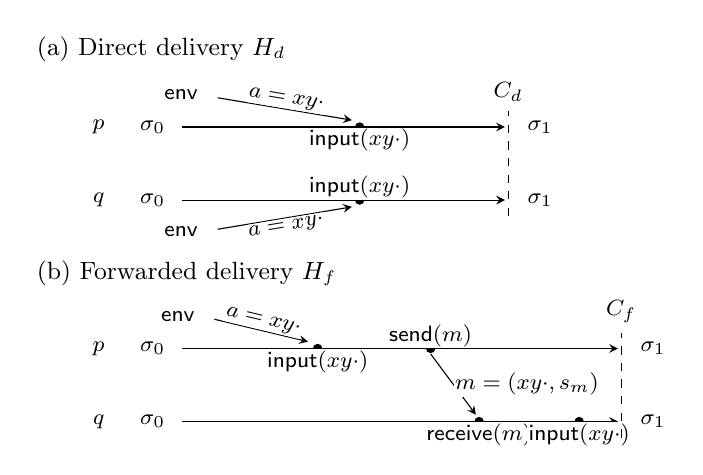
\begin{tikzpicture}[x=.82cm,y=.58cm,>=stealth,
                      every node/.style={font=\footnotesize}]
    % Direct delivery.
    \node[anchor=west,font=\small] at (-1,7.2) {(a) Direct delivery $H_d$};
    \node[anchor=east] at (.35,5.5) {$p$};
    \node[anchor=east] at (.35,3.9) {$q$};
    \node[anchor=west] at (.6,5.5) {$\sigma_0$};
    \node[anchor=west] at (.6,3.9) {$\sigma_0$};
    \draw[->] (1.4,5.5) -- (6.4,5.5);
    \draw[->] (1.4,3.9) -- (6.4,3.9);
    \fill (4.15,5.5) circle (1.7pt);
    \fill (4.15,3.9) circle (1.7pt);
    \node[below,fill=white,inner sep=.5pt] at (4.15,5.5)
      {$\mathsf{input}(xy\cdot)$};
    \node[above,fill=white,inner sep=.5pt] at (4.15,3.9)
      {$\mathsf{input}(xy\cdot)$};
    \node[anchor=east] at (1.8,6.2) {$\mathsf{env}$};
    \node[anchor=east] at (1.8,3.2) {$\mathsf{env}$};
    \draw[->] (1.95,6.14) -- node[midway,above,sloped,fill=white,inner sep=.5pt]
      {$a=xy\cdot$} (4.03,5.65);
    \draw[->] (1.95,3.26) -- node[midway,below,sloped,fill=white,inner sep=.5pt]
      {$a=xy\cdot$} (4.03,3.75);
    \draw[dashed] (6.45,3.55) -- (6.45,5.85);
    \node[above] at (6.45,5.85) {$C_d$};
    \node[anchor=west] at (6.6,5.5) {$\sigma_1$};
    \node[anchor=west] at (6.6,3.9) {$\sigma_1$};

    % Forwarded delivery.
    \node[anchor=west,font=\small] at (-1,2.3) {(b) Forwarded delivery $H_f$};
    \node[anchor=east] at (.35,.65) {$p$};
    \node[anchor=east] at (.35,-.95) {$q$};
    \node[anchor=west] at (.6,.65) {$\sigma_0$};
    \node[anchor=west] at (.6,-.95) {$\sigma_0$};
    \draw[->] (1.4,.65) -- (8.15,.65);
    \draw[->] (1.4,-.95) -- (8.15,-.95);
    \node[anchor=east] at (1.75,1.35) {$\mathsf{env}$};
    \draw[->] (1.9,1.29) -- node[midway,above,sloped,fill=white,inner sep=.5pt]
      {$a=xy\cdot$} (3.35,.8);
    \fill (3.5,.65) circle (1.7pt);
    \node[below,fill=white,inner sep=.5pt] at (3.5,.65)
      {$\mathsf{input}(xy\cdot)$};
    \fill (5.25,.65) circle (1.7pt);
    \node[above,fill=white,inner sep=.5pt] at (5.25,.65)
      {$\mathsf{send}(m)$};
    \fill (6.0,-.95) circle (1.7pt);
    \node[below,fill=white,inner sep=.5pt] at (6.0,-.95)
      {$\mathsf{receive}(m)$};
    \draw[->] (5.25,.53) -- node[midway,right,fill=white,inner sep=.5pt]
      {$m=(xy\cdot,s_m)$} (5.95,-.8);
    \fill (7.55,-.95) circle (1.7pt);
    \node[below,fill=white,inner sep=.5pt] at (7.55,-.95)
      {$\mathsf{input}(xy\cdot)$};
    \draw[dashed] (8.2,-1.3) -- (8.2,1.0);
    \node[above] at (8.2,1.0) {$C_f$};
    \node[anchor=west] at (8.35,.65) {$\sigma_1$};
    \node[anchor=west] at (8.35,-.95) {$\sigma_1$};
  \end{tikzpicture}
  \caption{Two distinct histories from $\sigma_0=(x\cdot\cdot,R_0)$ to
  $\sigma_1=(xy\cdot,R_1)$.  The relations $R_0$ and $R_1$ are, respectively, the tables in panels (a) and (b) of
  Figure~\ref{fig:election-frames}.  The environment supplies cumulative input $a=xy\cdot$.  The strategy
  computes $\mathsf{advance}(x\cdot\cdot,xy\cdot)=xy\cdot$; the resulting
  $\mathsf{input}(xy\cdot)$ is the participant event.  In (b), $q$ computes
  the $\mathsf{advance}$ upon receiving $m=(xy\cdot,s_m)$.  Vertical dashed lines are consistent cuts.}
  \label{fig:history-projection}
\end{figure}

The figure shows why we need a transition projection.  A Lamport history
records sends, receives, and strategy state even when they make no difference
to the specification state.  The projection filters each participant's history
to the transitions that determine that state.

\begin{definition}[Transition projection and state endpoint]
\label{def:semantic-projection}
For a consistent cut $C$ and participant $p$, list the events of $C$ assigned
to $p$ in local order.  Its \emph{transition projection} $\pi_p(C)$ keeps input,
preparation, and exposure events in that order and deletes sends and receives.
A receive may update strategy state and lead the strategy to
compute a later input event, but it does not directly change the specification state.
We consider only pairs $(H,C)$ for which each $\pi_p(C)$ is a defined
transition sequence from $\sigma_0(i_p)$ and every input event caused by an
arrival or receive has the target computed by $\mathsf{advance}$.  Write
$\sigma_p(C)$ for the final specification state of $\pi_p(C)$.  The
\emph{state endpoint} of the cut is the vector
        \begin{equation}
  \operatorname{end}(H,C)=(\sigma_p(C))_{p\in P}.
  \label{eq:semantic-endpoint}
        \end{equation}
Every transition projection is a run or a run prefix under the history's
commitment basis.  A pending-exposure prefix has the unique completion required
by the history definition before applying a run-confluence result.
\end{definition}

At both cuts in Figure~\ref{fig:history-projection}, each local projection is
$\mathsf{input}(xy\cdot)$, so
$\operatorname{end}(H_d,C_d)=\operatorname{end}(H_f,C_f)
=(\sigma_1,\sigma_1)$.  Projection erases the delivery path while retaining
its effect on the participant states.

State endpoints determine which state transformations are enabled next.  Equal
endpoints have the same applicable transformations and effects because each is
a partial function of the specification state.  They need not determine the
same future history: participants and the environment may have observed
different exposures, and those observations may influence later inputs or
strategy choices.

\paragraph{Confluence of a history.}
At a consistent cut $C$, the participants may hold different specification states
$(\sigma_p(C))_{p\in P}$.  Confluence asks whether their local paths can be
brought to the same later state at every input that combines their current
inputs.
Formally, first complete every pending exposure at $C$.  Let $j$ be a common
refinement of the resulting participant inputs.  The history $H$ is
\emph{confluent at $C$ and $j$} when it has a further extension using input
events and complete exposure sequences in which every participant reaches the
same specification state
$\sigma_j=(j,R)$; equivalently, the new cut has state endpoint
$(\sigma_j)_{p\in P}$.  This is an existence claim about transitions, not a
claim that a protocol delivers $j$, communicates, or terminates.

\subsection{Distributed Consistency}
\label{sec:distributed-consistency}

Confluence is a property at one cut and common input refinement.  Distributed
Consistency requires it at every cut of every history under the canonical
commitment basis.

\begin{definition}[Distributed Consistency]
\label{def:distributed-consistency}
An ordered specification has \emph{Distributed Consistency} when, for every
finite participant set, history $H$ under the canonical commitment basis, and
consistent cut $C$, $H$ is
confluent at $C$ and every common refinement of
the participants' current inputs.
\end{definition}

Distributed Consistency is the history-level reading of consistency.  The
next proposition states their exact relationship; its short proof is also why
the run formulation remains useful.

\begin{proposition}[Consistency and Distributed Consistency]
\label{prop:distributed-consistency}
An ordered specification is consistent if and only if it has Distributed
Consistency.
\end{proposition}

\begin{proof}
At any cut, take the unique completion of each pending exposure.  The resulting
projections are a finite set of runs under the canonical commitment basis, so
Consistency implies their confluence from those completed endpoints; together
with the pending exposures, this is an extension from the original cut.
Conversely, place any finite set of such runs in a message-free
history, one per participant, supplying each
input target $j$ as the cumulative arrival $a=j$.
Equation~\ref{eq:cumulative-advance} records each such step.  Distributed
Consistency at the final cut gives run confluence.
\end{proof}

Combining Proposition~\ref{prop:distributed-consistency} with Functional CALM,
a functional specification has Distributed Consistency exactly when it is
monotone.  This distributed reading does not depend on output choice.  We next
make that orthogonal extension to ambiguous specifications.
